\chapter{Investment Banks}

These notes follow Robert J. Shiller's lecture on investment banks, together with Jan Fugner's later classroom discussion, and have been curated by LazyingArt LLC. The lecture proceeds in a clear sequence. We begin by separating investment banking from consulting, trading, and commercial banking. We then ask what economic function justifies the investment bank's existence at all, and the answer is a trust technology built around underwriting, due diligence, and reputation. From there the lecture moves to the regulatory boundary between deposit banking and securities business, then to the sharpest analytical point of the chapter: shadow banking, repo funding, and the run on Lehman Brothers. Only after that does the lecture turn inward, to the analyst's world of models and pitch books, and finally outward again, to Facebook, the social graph, and the measurement of advertising.

\section{Investment Banking as a Distinct Business}

We begin, as the lecture does, by defining investment banking through contrast. An investment bank helps a corporation, a government, or some other incorporated entity create securities and raise capital. It may help issue stock; it may help issue bonds. What matters is that it stands at the point where an issuer turns a financing need into a security sold to outside investors.

\begin{definition}
An investment bank, in the narrow sense used at the start of the lecture, is an institution that helps issuers create and place securities. A pure investment bank does not accept deposits.
\end{definition}

This immediately separates the business from commercial banking. One does not go to a pure investment bank to open a checking account or a savings account. The separation from consulting is subtler. The investment bank often gives advice about corporate strategy, financing choice, or the timing of an offering. But it is not a pure consultant, because it does not merely advise. It also helps bring the money.

The lecture then narrows the definition into underwriting. If a company wants to issue shares, the investment bank identifies likely buyers, manages the issuance, and in effect stands behind the sale. The lecture distinguishes several common objects:

\begin{itemize}
\item An initial public offering is the first public issuance of a firm's shares.
\item A seasoned offering is an additional issuance by a firm whose shares already trade publicly.
\item In a bought deal, the bank purchases the securities itself and resells them.
\item In a best-efforts offering, the bank does not buy the securities, but undertakes to place them as successfully as it can.
\end{itemize}

The lecture also insists that investment banking is not the same thing as trading. The trader buys and sells. The investment banker, in the idealized picture presented here, helps an institution do something that it could not easily do on its own: issue securities, finance a project, or carry out a merger.

\subsection{Question \& Answer}

\paragraph{Question.} Why is investment banking not just consulting with better contacts, or just another kind of banking?

\paragraph{Answer.} Because the bank is performing a different economic task. A consultant may diagnose a problem and offer advice. A commercial bank may take deposits and make loans. The investment bank, by contrast, organizes access to securities markets. It advises, but it also helps create and place claims. It is therefore neither pure advice nor pure deposit intermediation. In the lecture's vocabulary, it is a business of helping others create securities.

\section{Trust, Due Diligence, and Reputation}

At this point the lecture asks a deeper question. Why should an outside investor trust a new issue? The answer is not simply that a prospectus has been filed or that the issuer wants money. Shiller reframes the underwriting function as a solution to a moral hazard problem.

\begin{definition}
The moral hazard problem in this setting is that insiders may know more than outsiders about the true state of the issuing firm and may try to sell securities before adverse information becomes public.
\end{definition}

The lecture makes the point vividly. If a firm knows that it is headed toward bankruptcy, why should it not issue shares before the public understands the situation? The investment bank exists partly to block exactly that sort of opportunism. It performs due diligence. It checks the issuer. It screens. Then, if the bank is willing to stand behind the issue, investors infer that a reputable intermediary has put its name on the line.

So the central asset of investment banking is reputation. The lecture returns to this idea repeatedly: investment banking is built around trust. That is why Shiller emphasizes manner, cultivation, and the visible marks of seriousness. These are not presented merely as matters of taste. They are institutional supports for credibility.

The lecture then turns to Goldman Sachs as an example of a bank whose public image and internal culture were long tied to this reputation-based business. Shiller uses Charles Ellis's history of Goldman Sachs to draw out a cluster of principles: clients first, assets understood as people, capital, and reputation, loyalty to the firm, discretion, and avoidance of unnecessary publicity. We should not read this section as a generic corporate portrait. The lecture's point is sharper. In a business where the intermediary must persuade others that an issue is sound, character and institutional culture become economic inputs.

\subsection{Question \& Answer}

\paragraph{Question.} Why does underwriting depend so heavily on reputation?

\paragraph{Answer.} Because the issue itself does not speak. Someone must certify, implicitly or explicitly, that the issuer has been examined and that the offering can be taken seriously. Reputation is valuable precisely because it can be lost. The investment bank's name is therefore a scarce asset, and due diligence is the mechanism by which that asset is defended.

\section{Separation, Repeal, and Partial Restoration}

The lecture next shifts from institutional culture to legal structure. Once we see that investment banks traffic in reputation and capital-market access, the next question is where the regulatory boundary should be drawn. Shiller answers historically.

In 1933 the Glass-Steagall framework separated commercial banking from investment banking. In the lecture's logic this made sense for a simple reason. If the government is going to insure deposits through the FDIC, then it cannot remain indifferent to the risks taken by the insured institution. The state, having guaranteed deposit liabilities, acquires a reason to prevent insured banks from entering activities thought to be especially dangerous. In the lecture, investment banking is presented as one such dangerous business.

Shiller uses the Morgan example to dramatize the split. The important point is not family genealogy; it is institutional separation. The old mixed structure could not continue unchanged. Commercial banking and investment banking were pushed apart.

The lecture then moves to the repeal of that separation in 1999, when the United States moved toward universal banking. Shiller's sequence is important. He does not present repeal as a purely ideological event. He presents it as a competitive response to Europe and other jurisdictions where banks had long conducted both lines of business under one roof.

After the crisis, however, the older question returned. If insured banks are once again entangled with market activity, has the state recreated the very problem it had tried to avoid? The lecture does not answer by calling for a full restoration of Glass-Steagall. Instead it turns to partial measures.

The first is the Volcker Rule, which Shiller presents as a partial return to separation. Commercial banks are not to engage in proprietary trading, and they are restricted in their ownership of hedge funds and private-equity vehicles. The second is the Lincoln amendment, which the lecture associates with an attempt to deny certain swap-dealing activities the support of the federal safety net. The exact statutory details are secondary here. The analytical point is that the government tries to separate activities not by splitting the bank entirely in two, but by restricting the combination of insured funding and speculative trading.

\subsection{Question \& Answer}

\paragraph{Question.} Why separate commercial banking and investment banking, and why only partially restore that boundary later?

\paragraph{Answer.} The first separation follows from deposit insurance. Once deposits are guaranteed, the state becomes exposed to bank risk and has an incentive to restrict that risk. The later partial restoration reflects a different world: universal banking had already returned, so regulation aimed not at complete institutional divorce, but at blocking especially dangerous combinations such as insured banking plus proprietary speculation.

\section{Shadow Banking, Repos, and the Run on Lehman Brothers}

Here the lecture reaches its analytical core. The decisive move is to stop treating legal labels as economically decisive. A firm may not accept deposits and yet may still fund itself in a way that makes it vulnerable to the same logic as a commercial-bank run.

\begin{definition}
A shadow bank is an institution that performs economically bank-like functions without being regulated as a commercial bank.
\end{definition}

The lecture then introduces the repo market.

\begin{definition}
A repo, or repurchase agreement, is a transaction in which one party effectively borrows cash by selling a security today and agreeing to repurchase it later.
\end{definition}

The lecture gives this mechanism verbally, not algebraically, so we write the usual notation with caution.

\begin{remark}
The next equations are standard formalizations of the mechanism described in the lecture, not transcriptions of a board derivation.
\end{remark}

\begin{align}
\text{cash raised today} &= P_0, \\
\text{cash paid back at maturity} &= P_1, \\
\text{financing cost} &= P_1 - P_0, \\
r_{\text{repo}} &= \frac{P_1-P_0}{P_0}.
\end{align}

Economically, the transaction behaves like a short-term collateralized loan. Shiller's point is that it also behaves like runnable short-term funding:

\begin{equation}
\text{repo funding} \approx \text{short-term runnable deposit-like funding}.
\end{equation}

The crucial difference is not in the logic of the run but in the identity of the lender. In the commercial-bank case, the lender is the small depositor. In the repo case, the lender is more likely to be a large institutional investor. But in both cases short-term funding can disappear quickly.

\subsection{Question \& Answer}

\paragraph{Question.} How can a firm that does not accept deposits still suffer something that looks exactly like a bank run?

\paragraph{Answer.} Because the run is a funding phenomenon, not merely a legal category. If a firm's liabilities are very short term and lenders can refuse to renew them, then fear can force an immediate contraction in funding. Deposits are one way to create that vulnerability; repo borrowing is another.

We can state the liquidity logic compactly:

\begin{equation}
\text{maturing repo not renewed}=\text{asset sales}+\text{new funding}.
\end{equation}

This is the balance-sheet pressure that drives the lecture's discussion of Lehman Brothers. If the maturing repo is not rolled over, the bank must either find replacement funding or sell assets. If asset values are already falling, forced sales intensify the crisis.

\paragraph{Derivation of the run mechanism.}
\begin{enumerate}
\item Lehman finances a large stock of assets through short-term repos.
\item The housing downturn reduces the value of mortgage-related and subprime-linked assets.
\item Repo lenders become uncertain about the quality of the bank's collateral and balance sheet.
\item They refuse to renew maturing repos.
\item Funding disappears faster than assets can be sold at acceptable prices.
\item The institution faces the economic equivalent of a bank run.
\end{enumerate}

\begin{figure}
\centering
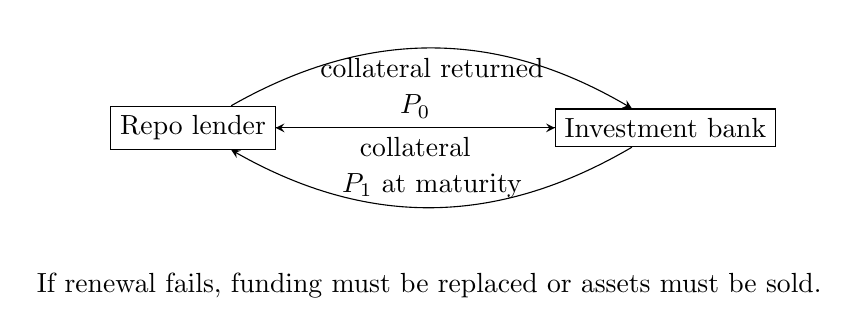
\begin{tikzpicture}[>=stealth]
\node[draw, rectangle] (lender) at (0,0) {Repo lender};
\node[draw, rectangle] (bank) at (6,0) {Investment bank};

\draw[->] (lender) -- node[above] {$P_0$} (bank);
\draw[->] (bank) -- node[below] {collateral} (lender);

\draw[->] (bank) to[bend left=30] node[above] {$P_1$ at maturity} (lender);
\draw[->] (lender) to[bend left=30] node[below] {collateral returned} (bank);

\node at (3,-2) {If renewal fails, funding must be replaced or assets must be sold.};
\end{tikzpicture}
\caption{Transcript-based reconstruction of repo funding.}
\end{figure}

The lecture then applies this structure to Lehman Brothers. Lehman, though a pure investment bank in the legal sense, had become economically bank-like because it financed proprietary positions with short-term repos. When confidence broke, the failure to roll those positions was a run. The lesson drawn in the lecture is that shadow banking cannot be understood simply by asking whether deposits are present. We must ask what kind of liabilities the institution has issued and how quickly they can disappear.

\section{Inside the Investment Banking Division}

Only after this macro-institutional analysis does the lecture turn to Jan Fugner. That sequencing matters. We now understand what the institution is doing in the financial system; Jan explains what it feels like to work inside it.

His first major correction is sociological and technical at once. The business may be described in public as relationship-driven, but at the junior level it is model-driven. The analyst builds operating models, transaction models, and valuation models; gathers information; turns that information into polished pitch books; and then helps carry the transaction through lawyers, accountants, counterparties, and clients.

The lecture gives the core hierarchy in the simplest possible way:

\begin{equation}
\text{Analyst}\to\text{Associate}\to\text{VP}\to\text{MD}.
\end{equation}

The point of the hierarchy is not ceremonial. On a lean deal team, perhaps one person at each of these ranks, responsibility can move upward and downward quickly. The analyst is not merely a spreadsheet mechanic. Once the bank wins a mandate, the analyst becomes part of the organizing principle that keeps the deal moving.

\subsection{Question \& Answer}

\paragraph{Question.} Why is investment banking presented as a relationship business but experienced, at the junior level, as a modeling business?

\paragraph{Answer.} Because the relationship is what wins access, but the model is what allows the bank to speak credibly once it has access. Senior bankers cultivate clients and boards. Junior bankers build the numerical and documentary machinery that makes advice precise enough to be used.

Jan's description of the work is especially useful because it refuses false glamour. There is little tolerance for numerical error. The analyst must get the details right. The discipline resembles engineering in this restricted but important sense: one does not have much flexibility to be wrong.

\paragraph{A typical analyst workflow.}
\begin{enumerate}
\item Build models describing the client and comparable firms.
\item Extract implications for financing, valuation, or transaction structure.
\item Present the result in a pitch book or other deal materials.
\item Once the mandate is won, coordinate execution across accountants, lawyers, clients, and counterparties.
\end{enumerate}

Jan also gives the inside tempo of the debt boom. Private-equity recruiting was so feverish that analysts could be interviewed and committed to post-banking jobs long before their formal start dates. Transactions arrived at such scale and frequency that people spoke of ``Merger Mondays,'' with very large deals announced at the start of the week. Even financial institutions, already highly levered, came to be discussed as leveraged-buyout candidates. This is the practitioner's counterpart to Shiller's earlier institutional story: the boom was real, exuberant, and in retrospect unstable.

The lecture briefly lightens the tone with the discussion of ``deal toys,'' but even there the underlying point is not frivolous. Finance has its own ritual objects, and the analyst's world mixes exhaustion, competition, precision, and a strange residue of play. The narrative then returns quickly to the crisis chronology: Bear Stearns, Merrill Lynch, Lehman, and then the conversion of Goldman Sachs and Morgan Stanley into commercial-bank holding companies. That sequence marks the end of the old pure-investment-bank era on Wall Street.

\section{From Banking to Technology: Social Graphs and Advertising Metrics}

Jan's move to Facebook might look, at first, like a digression. In fact it extends the lecture's larger theme that finance and technology both reward rigorous structure. The objects change, but the style of reasoning does not.

He describes Facebook's strategy as mapping a social graph. Again, the lecture gives the idea verbally, so we write the minimal notation cautiously.

\begin{remark}
The graph notation below is a clean formalization of Jan Fugner's description, not notation stated in the lecture itself.
\end{remark}

\begin{equation}
G=(V,E),
\end{equation}
where vertices represent users, and where one may enrich the picture to include objects, pages, or products:
\begin{equation}
G=(U\cup O,E).
\end{equation}

The lecture's intuition is that information travels along edges: who knows whom, who likes what, who has shown affinity for which product. This is not yet a theorem. It is an organizing picture. But it is a mathematically meaningful one.

The lecture then turns to click-through rate, which \emph{is} stated numerically and can be written directly:

\begin{equation}
\mathrm{CTR}=\frac{\text{clicks}}{\text{impressions}}.
\end{equation}

\paragraph{Worked example.}
If an advertisement is shown $100$ times and receives one click, then
\begin{equation}
\mathrm{CTR}=\frac{1}{100}=1\%.
\end{equation}

This is the lecture's clearest explicit numerical example. But Jan immediately resists the temptation to turn CTR into a universal metric. The reason is the marketing funnel:

\begin{equation}
\text{awareness}\to\text{affinity}\to\text{consideration}\to\text{purchase}\to\text{repeat purchase}.
\end{equation}

At the bottom of the funnel, where the user is already searching for a product and comparing vendors, clicking can be a natural proxy for progress toward purchase. Higher in the funnel, however, advertising may be trying to create awareness or affinity rather than immediate action. Then other metrics may be needed.

\subsection{Question \& Answer}

\paragraph{Question.} Why is click-through rate only one metric, and why does ``thinking like an engineer'' matter outside engineering?

\paragraph{Answer.} CTR measures one kind of response: direct clicking. But the lecture's funnel makes clear that different stages of persuasion require different measures. If the objective is awareness, a non-click measure may be more informative. If the objective is immediate purchase, CTR may be highly relevant. The engineering analogy enters because what matters is not the industry label but the discipline of reasoning: define the object, define the objective, choose the measurement that matches the objective, and be explicit about what the data can and cannot show.

The lecture closes in this broader register. Jan argues that one does not need to be a software engineer to contribute in a technology company, but one does need to think rigorously. Shiller then broadens the point further: finance and engineering both design devices. In finance the device may be a security, an institutional arrangement, or a funding structure; in technology it may be a platform, an advertising mechanism, or an experiment. In both cases serious work requires formal discipline.

\section{Summary}

The lecture begins with a distinction and ends with an analogy. First we distinguish investment banking from consulting, trading, and commercial banking. Then we see that its core economic function is to support the creation and placement of securities through underwriting, due diligence, and reputation. The crisis material sharpens that picture by showing that legal form is not enough: a pure investment bank can still become economically bank-like if it funds itself through runnable short-term liabilities such as repos. Jan Fugner's account then turns the outside view inward. Junior banking is a world of models, pitch books, and execution discipline, set against the exuberance of the debt boom and the abrupt end of the old Wall Street structure. The final movement to Facebook does not abandon the lecture's analytical spirit. It shows instead that graph structure, measurement, and disciplined inference survive the shift from underwriting and repos to social networks and advertising.